\section{Quantitative Aspekte}

% TODO: Mehr und bessere Beispiele, generelle Überarbeitung (VL-Folien)

\subsection{Motivation}
\begin{frame}{Laufzeiten}
	Wir interessieren uns für Laufzeiten von Algorithmen.\\
	Aber wie sollen wir die messen?\\ \pause
	Problem: Rechenzeit auf einem Supercomputing-Cluster nicht mit Rechenzeit auf einem IoT-Chip in der Waschmaschine vergleichbar.\\
	
	\bigskip \pause
	Daher: Zählen der \enquote{ausgeführten Operationen} in Abhängigkeit von der Problemgröße $n$.\\
	Meistens interessiert vor allem der Worst-Case.
\end{frame}

\begin{frame}{Abschätzung}
	Genaue Abschätzungen sind oftmals \textit{sehr schwierig}.\\
	Aber oftmals auch \textit{sehr uninteressant}.\\
	Konstante Faktoren z.B. sind durch die ständigen Verbesserungen bei Prozessoren oftmals für die Praxis irrelevant.\\
	
	\bigskip \pause
	Uns interessiert vor allem das Verhalten für \textit{sehr große} Instanzen.
\end{frame}

%% -----------------------------------------------------------------------------

\subsection{Definitionen}
\begin{frame}{Asymptotisches Wachstum}
	\begin{Definition}
		Zwei Funktionen $f,g: \N_0 \to \R_0^+$ wachsen asymptotisch gleich schnell, wenn es zwei Konstanten $c, c' \in \R^+$ gibt, so dass gilt $$\exists n_0 \in \N_0: \ \forall n \geq n_0: \ c \· f(n) \leq g(n) \leq c' \· f(n) $$
		Man schreibt dafür 
		\begin{align*}
			f &\asymp g \\
			\textbf{oder} \quad f(n) &\asymp g(n) \quad \text{{\small (Ja, das ist auch OK!)}}  
			% Hashtag: „n^2“ ist ein Term und keine Funktion etc... Man müsse doch [n \mapsto n^2] schreiben... VL erlaubt ersteres aber auch.
		\end{align*}
	\end{Definition} \pause
	Diese Relation ist eine Äquivalenzrelation!
\end{frame}

\begin{frame}{Landau-Notation I}
	\begin{Definition}
		$\Theta(f)$ ist die Menge aller Funktionen $g$, die asymptotisch genauso schnell wachsen wie $f$, also $$\Theta(f) := \{ g \mid f \asymp g \}$$
	\end{Definition}
	
	\medskip
	\only<1|handout:1>{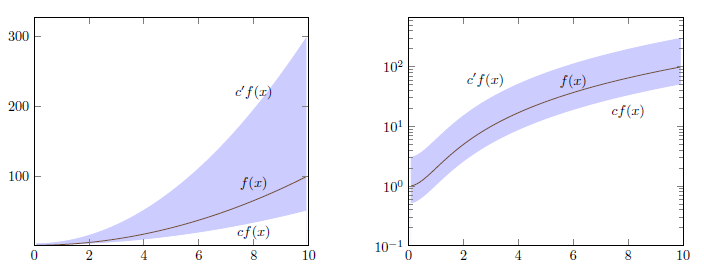
\includegraphics[scale=0.6]{laufzeit/theta1}}
	\only<2|handout:2>{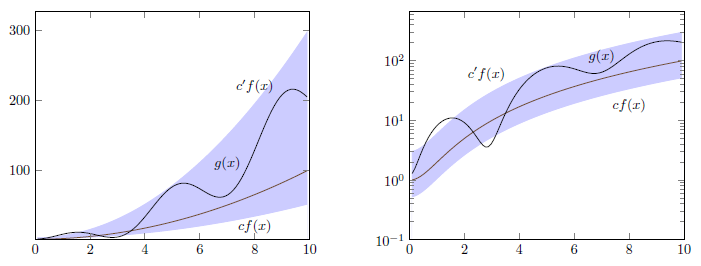
\includegraphics[scale=0.6]{laufzeit/theta2}}
\end{frame}

\begin{frame}{Beispiel}
	$$f(n) := 2 \cdot n^2 + n \qqquad g(n) := n^2$$
	\medskip
	Zeige: $ f \in \Th{g} $.\\ \pause
	Wir suchen $n_0, c, c'$ mit $\forall n \geq n_0: \ c \· g(n) \leq f(n) \leq c' \· g(n) $ \pause
	\medskip
	
	Sei $n \geq 1$, so gilt:\\\pause
	$f(n) = 2 \cdot n^2 + n \leq 2 \cdot n^2 + n^2 = 3 \cdot n^2$ und \\\pause
	$f(n) = 2 \cdot n^2 + n \geq 2 \cdot n^2$
	\medskip
	
	Mit $c := 2$, \, $c' := 3$,\, $n_0 := 1$ ist die Bedingung erfüllt. \qed \pause
	
	\begin{block}{Quiz}
		\TrueQuestion{$n^{100} + 10^9 n^{99} \in \Th{n^{100}}$}
		\FalseQuestion{$2^n \in \Th{n^2}$}
	\end{block}
\end{frame}

\begin{frame}{Beispiel 2}
	\textbf{Behauptung:} \quad $ [n \mapsto \sin(n) + 2] \elem \Th{n \mapsto 1} $ \\ \medskip \pause
	\textbf{Beweis:} \quad Wähle $c := 1, \, c' := 3, \, n_0 := 0$.  \quad Dann gilt $\forall n \geq n_0$: \\
	\begin{align*}
	c \· 1 = 1 &\leq \sin(n) + 2 \leq 3 = c' \· 1 \\
	\text{\Gdw} \qquad  -1 &\leq \sin(n) \leq 1. \qed
	\end{align*}
	\pause
	\Impl Der Sinus ist also „ungefähr“ konstant\only<handout>{ (wenn man seine Brille absetzt \smiley)}.
\end{frame}

\begin{frame}{Asymptotisches Wachstum}
	\begin{Definition}
		Für zwei Funktionen $f,g: \N_0 \to \R_0^+$ definiert man:
		$$g \preceq f \Gdw \exists c \in \R^+ \ \exists n_0 \in \N_0 \ \forall n \geq n_0: \ g(n) \leq c \· f(n)$$
		$$g \succeq f \Gdw \exists c \in \R^+ \ \exists n_0 \in \N_0 \ \forall n \geq n_0: \ g(n) \geq c \· f(n)$$
		(Schreibe analog auch $g(n) \preceq f(n)$ etc.)
	\end{Definition} \pause
	Diese Relationen sind \textbf{keine} Äquivalenzrelationen!
\end{frame}

\begin{frame}[t]{} % erased title due to \includepdf madness... I guess it's not that important anyway. Tags: fake title faketitle include pdf frametitle
	\fakeframetitle{Landau-Notation II}
	\begin{Definition}
		$\Oh{f}$ ist die Menge aller Funktionen $g$, die asymptotisch höchstens so schnell wachsen wie $f$, also $$\Oh{f} := \{ g \mid g \preceq f \}$$
		$\Om{f}$ ist die Menge aller Funktionen $g$, die asymptotisch mindestens so schnell wachsen wie $f$, also $$\Om{f} := \{ g \mid g \succeq f \}$$
	\end{Definition} \pause
	\impl $O$ ist eine Abschätzung nach oben. $\Omega$ ist eine Abschätzung nach unten.
\end{frame}


\setbeamercolor{background canvas}{bg=}

\includepdf[pages=15]{U11.pdf}

\begin{frame}{Eine katastrophale Schreibweise}
	Manchmal (häufig) sieht man auch das, \textbf{NICHT VERWENDEN}:
	$$f = \Theta(g) \qquad h = \Oh{n^3} \qquad k = \Omega(f + g)$$
	\pause
	Dabei ist das $=$ immer als $\in$ zu verstehen!
\end{frame}

\begin{frame}{}
	Ordnet folgende Funktionen nach asymptotischem Wachstum an:
	\begin{itemize}
		\item Identität $f(x) = x$
		\item Konstante Funktion $f(x) = c$
		\item Wurzel
		\item Exponentialfunktion
		\item Logarithmus
	\end{itemize}
\end{frame}

%% Übung: Asymptotische Visualisierungen verschiedener Funktionen
\setbeamercolor{background canvas}{bg=}

\includepdf[pages={5-10}]{U11.pdf}

%\begin{frame}
%	\frametitle{Grenzwertabschätzung}
%	Wir können das auch anders schreiben:
%	\begin{align*}
%	f \in O(g) \qquad &\iff & \qquad 0 \leq  \limsup \limits_{n \to \infty} \frac{f(n)}{g(n)} < \infty \\
%	f \in \Omega(g) \qquad &\iff & \qquad 0 < \liminf  \limits_{n \to \infty} \frac{f(n)}{g(n)} \leq \infty \\
%	f \in \Theta(g) \qquad & \iff & \qquad 0 <  \liminf  \limits_{n \to \infty} \frac{f(n)}{g(n)} \leq  \limsup \limits_{n \to \infty} \frac{f(n)}{g(n)} < \infty
%	\end{align*} \pause
%	Oftmals existiert sogar $\lim$ und wir können $\liminf$ und $\limsup$ vergessen!
%\end{frame}
%
%\begin{frame}{Satz von L'Hospital}
%	\begin{block}{Satz}
%		Gegeben sei $$ \limes{x\to x_0} \frac{f(x)}{g(x)} $$ mit $$ \limes{x\to x_0} f(x) = \limes{x\to x_0} g(x) = 0 \vee \limes{x\to x_0} f(x) = \limes{x\to x_0} g(x) = \infty $$ 
%		Dann gilt 
%		$$ \limes{x\to x_0} \frac{f(x)}{g(x)} = \limes{x\to x_0} \frac{f'(x)}{g'(x)}   $$ mit 
%		$$ f'(x_0) = \left. \frac{\partial f(x)}{\partial x} \right|_{x=x_0} $$ 
%	\end{block}
%\end{frame}
%
%\begin{frame}{Beispiele}
%	Gilt $$ \log n \in \O \left(\sqrt{n}\right) $$ \pause 
%	Betrachte
%	\begin{align*}
%		\limes{n\to\infty} \log n &= \infty \\
%		\limes{n\to\infty} \sqrt{n} &= \infty \\
%		\frac{\partial \log n}{\partial n} &= \frac{1}{n} \\
%		\frac{\partial \sqrt{n}}{\partial n} &= \frac{1}{2} \frac{1}{\sqrt{n}} \\
%		\limes{n\to\infty} \frac{\log n}{\sqrt{n}} &= \limes{n\to\infty} \frac{\frac{1}{n}}{\frac{1}{2} \frac{1}{\sqrt{n}}} \\
%		&= 2 \limes{n\to\infty} \frac{\sqrt{n}}{n}  = 2 \limes{n\to\infty} \frac{1}{\sqrt{n}} = 0 
%	\end{align*}
%\end{frame}

%\subsection{Beispiele}
%\begin{frame}{Polynome}
%	Betrachten wir zwei Polynome $f(n) = n^4 + n^3$ und $g(n) = n^2$: \\
%	Der Quotient $$\frac{f(n)}{g(n)} = \frac{n^4 + n^3}{n^2} = n^2 + n \to \infty$$ Also ist $\lim f/g > 0$ und damit $$g \in O(f) \qquad f \in \Omega(g)$$ aber $\lim f/g = \infty$ also $$f \not \in O(g) \qquad g \not \in \Omega(f)$$ und vor allem $$f \not \in \Theta(g)$$
%\end{frame}

\begin{frame}{Logarithmen}
	\only<handout:0>{Informatiker LIEBEN Logarithmen...\\}
	\begin{block}{Einige Rechenregeln}
		\begin{align*}
			a^{\log_a n} &= n\\
			\log_b n^a &= a \cdot \log_b n\\
			\log_b (n \cdot m) &= \log_b n + \log_b m\\
			a^{\log_b n} &= n^{\log_b a}
		\end{align*}
	\end{block}
\end{frame}

\begin{frame}{Logarithmen}
	\begin{block}{Lemma}
		$$a^{\log_b n} = n^{\log_b a}$$
	\end{block}

	\begin{block}{Herleitung}
		\begin{align*}
			a^{\log_b n} &= \left( b ^{\log_b a} \right) ^{\log_b n}\\
						 &= b^{\log_b a \, \cdot \, \log_b n}\\
						 &= \left( b^{\log_b n} \right) ^{\log_b a}\\
						 &= n^{\log_b a}
		\end{align*}
	\end{block}
\end{frame}

\begin{frame}{Logarithmen: Die Basis ist egal}
	\begin{block}{Lemma}
		$$ \log_a n \in \Th{\log_b n} $$
	\end{block}
	
	\begin{block}{Herleitung}
		Es gilt $$n = a^{\log_a n}$$ \pause
		Daraus ergibt sich: $$ \log_b n = \log_b \left(a^{\log_a n}\right) = \log_a n \; \cdot \log_b a $$ \pause 
		Setze $c = c' = \log_b a$, dann ist $$c \· \log_a n \leq \log_b n \leq c' \· \log_a n.$$
	\end{block}
\end{frame}

\begin{frame}{Rechenregeln (I)}
	Einige Rechenregeln im $O$-Kalkül
	\begin{itemize}[<+->]
		\item Für $a > 0$ ist $a \cdot f \in \Th{f}$ 
		\item Für Konstanten $c, d \geq 0$ gilt: \\ 
			\quad $f(n) \in \Oh{g(n)} \Impl f(n) + c \in \Oh{g(n) + d}$ \\
			\quad $f(n) \in \Om{g(n)} \Impl f(n) + c \in \Om{g(n) + d}$ \\
		\item Für $0 < a < b$ ist $n^a \preceq n^b$
		\item Für $a,b > 1$ ist $n^a \preceq b^n$ \qquad {\small (Exponentialfktnen. wachsen stärker als Polynome)}
		\item Für Polynome $f,g$ gilt: \\
			\quad $\mathop{\text{grad}} f = \mathop{\text{grad}} g \iff f \asymp g $
		\item Für $a,b > 0$ gilt $\log_a(n) \in \Theta(\log_b n)$
		
	\end{itemize}
\end{frame}


\begin{frame}{Rechenregeln (II)}
	Weitere Rechenregeln im $O$-Kalkül:
	\begin{itemize}[<+->]
		\item $f \in O(g) \iff g \in \Omega(f)$
		\item $\Theta(f) = O(f) \cap \Omega(f)$ und $f \asymp g \iff f \preceq g \wedge f \succeq g$ 
		\item $O(f_1) + O(f_2) = O(f_1 + f_2)$
		\item Wenn $g \in O(f)$, dann ist auch $O(g) \subseteq O(f)$ und $O(f + g) = O(f)$
	\end{itemize}
	
\end{frame}

%\subsection{Laufzeiten Angeben}
%
%\begin{frame}[fragile]
%	\frametitle{Algorithmus}
%		\verb+int x = 1;+ \\
%		\verb/for (int i = 0; i < n; i++) {/ \\
%		\verb+	x = a * x;+ \\
%		\verb+}+ \\
%		\verb+return(x);+ \\[1em]
%		 \pause
%	Was tut der? \pause Welche Laufzeit hat er?
%\end{frame}
%
%\begin{frame}[fragile]
%	\frametitle{Laufzeiten}
%		\verb+int x = 1;+ \\ \pause $O(1)$ \\ \pause
%		\verb/for (int i = 0; i < n; i++) {/ \\  \pause $O(1), O(1)$ \\ \pause
%		\verb+	x = a * x;+ \\  \pause $O(1)$ \\ \pause
%		\verb+}+ \\  \pause $n$-mal \\ \pause
%		\verb+return(x);+ \\  \pause $O(1)$ \\ \pause
%		 \pause
%		$$O(1 + n + n + 1) = O(n)$$
%\end{frame}
